\chapter{Evaluatie}

\section{Preprocessing}

Om goede resultaten te verkrijgen bij actieherkenning, is het noodzakelijk om allereerst de gegevens te normaliseren. Belangrijke factoren zijn onder andere de positie van de persoon ten opzichte van de Kinect camera in zowel de horizontale, verticale en diepterichting, de schaal van de persoon zoals de lengte van de armen en benen, en de oriëntatie van de persoon ten opzichte van de camera. Voor de normalisatie is er een \textit{referentiejoint} nodig om te voorkomen dat er gewerkt wordt met absolute waarden. Deze rol wordt vervuld door de \textit{Spine Base Joint} $(\textbf{J}_{sb})$ aangezien deze de enigste joint is die geen kind is van een andere \textit{joints}. Een \textit{joint} $p$ is een ouder van een andere \textit{joint} $c$ als er een pad bestaat vanuit $\textbf{J}_{sb}$ naar $c$ waarbij de voorlaatste knoop op dit pad $p$ is. Figuur \ref{fig:skeleton_graph} toont de boomstructuur die deze relaties voorstelt.

%\begin{figure}[ht]
%	\centering
%	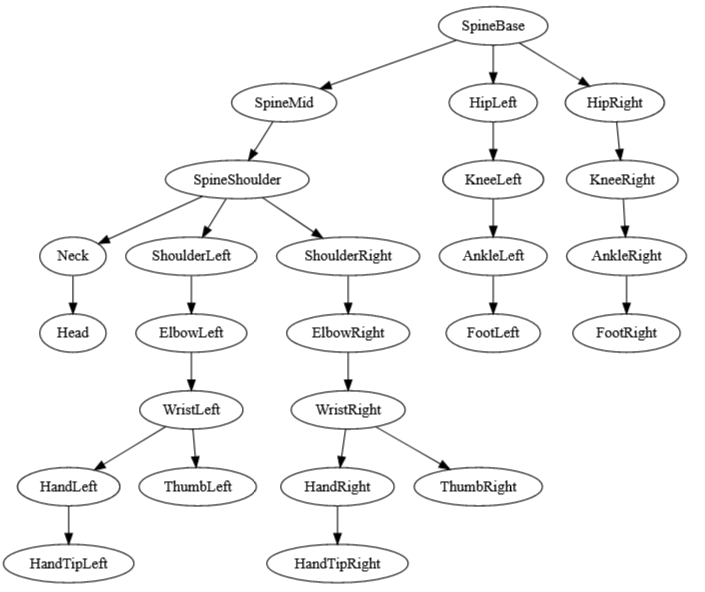
\includegraphics[width=0.7\textwidth]{skeleton_graph}
%	\caption{De \textit{joints} van de Kinect voorgesteld in een boomstructuur.}
%	\label{fig:skeleton_graph}
%\end{figure}


De volgende drie onderdelen bespreken de verschillende stappen van de \textit{preprocessing} fase.

\subsubsection{Plaats-invariantie}
Om ervoor te zorgen dat een persoon zich eender waar kan bevinden in het bereik van de Kinect camera, zonder invloed te hebben op de classificatie, wordt een translatie uitgevoerd zodat $\textbf{J}_{sb}$ zich in de oorsprong bevindt. Voor elke joint $\textbf{J}_i$ wordt zijn bijhorende puntvector $\textbf{P}_i$ aangepast via volgende bewerking:
$$\textbf{P}_i' = \textbf{P}_i - \textbf{P}_{sb}$$



\subsubsection{Rotatie-invariantie}
Een persoon kan verschillende oriëntaties aannemen ten opzichte van de camera, maar toch dezelfde actie uitvoeren. Elke joint $\textbf{J}_i$ bevat een \textit{quaternion} $\textbf{Q}_i = b\textbf{i} + c\textbf{j} + d\textbf{k} + w$ die de oriëntatie codeert van die joint. Aangezien $\textbf{J}_{sb}$ de referentiejoint is, zou deze de \textit{reeële quaternion} moeten bedragen. Dit is de \textit{quaternion} waarbij $w = 1$ en $b = c = d = 0$. Dit is mogelijk via het product van tussen $\textbf{Q}_{sb}$ en zijn conjugatie  $\textbf{Q}_{sb}^* = -b\textbf{i} - c\textbf{j} - d\textbf{k} + w$. Voor elke joint $\textbf{J}_i$ moeten nu twee bewerkingen uitgevoerd worden, enerzijds op de quaternion van de joint en anderzijds op de  drie-dimensionale coördinaten, waarop reeds een translatie is op uitgevoerd.

De eerste bewerking wijzigt de quaternion $\textbf{Q}_i$ door het product $\textbf{Q}_i\textbf{Q}_{sb}^*$ te nemen:
$$\textbf{Q}_i'' = \textbf{Q}_i\textbf{Q}_{sb}^*$$
De multiplicatie van twee quaternionen noemt men het \textit{Hamilton product}, maar de bewerking volgt gewoon de distributieregel.

Enkel de oriëntaties aanpassen is niet voldoende. Ook moeten de drie-dimensionale coördinaten aangepast worden om de juiste vorm van het skelet te behouden. Dit komt neer op het roteren van de puntvector $\textbf{P}_i'$ via de rotatie beschreven door $\textbf{Q}_{sb}$. Dit vertaalt zich in
$$\textbf{P}_i'' = \textbf{Q}_{sb}\textbf{P}_i'\textbf{Q}_{sb}^*$$

\subsubsection{Schaal-invariantie}



\todo{toon figuur waarbij verschillende aanpassingen te zien zijn}

%\begin{figure}
%	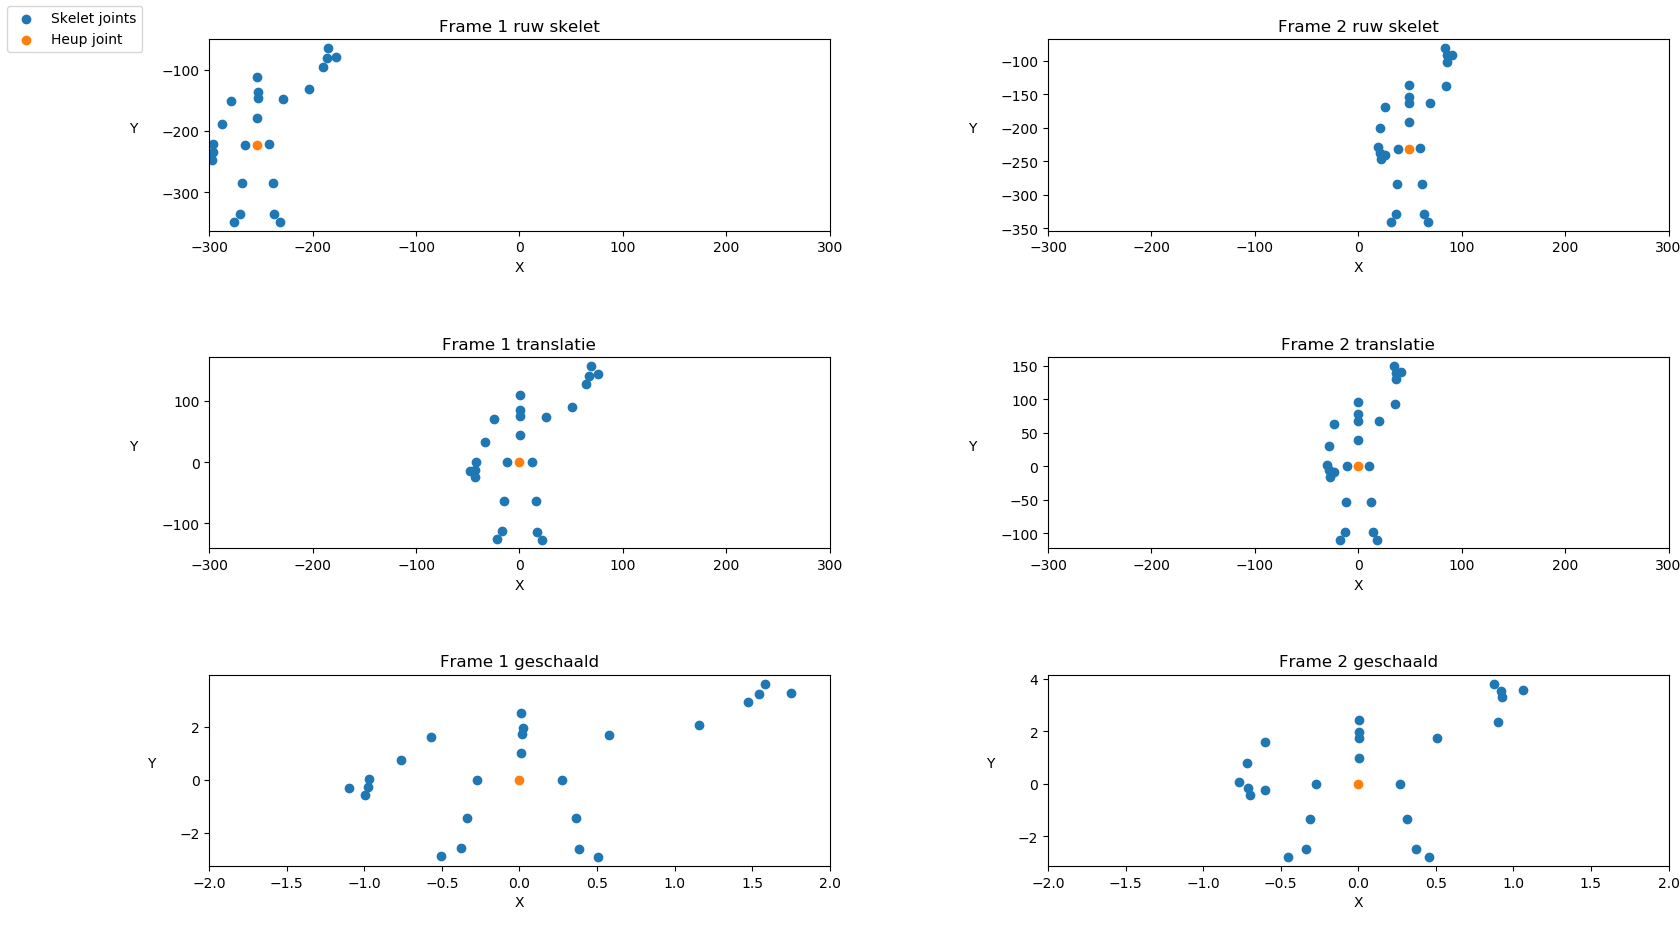
\includegraphics[width=\textwidth]{skeleton_preprocessing}
%	\caption{De impact van de verschillende preprocessing fasen op twee gelijkaardige acties. Hierbij is de oranje joint de \textit{Spine Base joint}.}
%	\label{fig:skeleton_preprocessing}
%\end{figure}

\section{Classifiers}
\label{ch:evaluatie}
De gebruikte dataset bestaat uit $x$ acties. De \textit{classifier} kan voor elk frame één van deze acties toekennen. Om de classifier te evalueren zou er een $x \times x$ frequentietabel opgesteld kunnen worden waarbij zowel de rijen als de kolommen gelabeld worden met de namen van de acties. De \textit{classifier} heeft dan een correcte classificatie uitgevoerd als de rij en kolom overeenkomen. Een vereenvoudigd voorbeeld is te zien op tabel \ref{table:example_evaluation}
\begin{table}[ht]
	\centering
	\begin{tabular}{| c | ccc |}
		\hline
				& zwaaien & bukken & springen \\
				\hline
		zwaaien & \textbf{5} & 2 & 0 \\
		bukken & 1 & \textbf{11} & 4 \\
		springen & 0 & 0 & \textbf{4} \\
		\hline
		
	\end{tabular}
	\caption{Een voorbeeld van een $3 \times 3$ frequentietabel.}
	\label{table:example_evaluation}
\end{table}

Het is echter moeilijk om hieruit eenvoudig relevante statistieken te berekenen. Het is daarom interessanter om de informatie van die tabel te aggregeren voor elke klasse om een zogenaamde \textit{confusion matrix} te bekomen. Op die manier wordt een binair classificatiemodel gesimuleerd. Tabel \ref{table:example_evaluation_aggregate} toont een voorbeeld van een \textit{confusion matrix} voor de klasse \texttt{bukken}. 
\begin{table}[ht]
	\centering
	\begin{tabular}{| c | cc |}
		\hline
		& bukken & niet-bukken \\
		\hline
		bukken & 11 (TP) & 5 (FP) \\
		niet-bukken & 2 (FN) & 9 (TN)\\
		\hline
	\end{tabular}
	\caption{Een}
	\label{table:example_evaluation_aggregate}
\end{table}

Er zijn nu 4 statistieken beschikbaar. Ten eerste is er het aantal keer dat de \textit{classifier} de actie 'bukken' heeft herkend terwijl het effectief bukken was. Dit wordt een \gls{ac:tp} genoemd. Ten tweede is er het aantal keer dat de \textit{classifier} herkent heeft dat de persoon niet aan het bukken was en dat het werkelijk zo niet was. Dit wordt een \gls{ac:tn} genoemd. Deze twee statistieken tonen aan wanneer de \textit{classifier} een juiste classificatie heeft gedaan voor deze specifieke actie. De overige twee statistieken zijn de \gls{ac:fp} en \gls{ac:fn} die respectievelijk het aantal keer aanduiden dat het bukken is terwijl het niet zo was, en dat het niet bukken is terwijl het wel zo was. \todo{dit moet voor elke klasse uitgevoerd worden}

Aan de hand van deze vier waarden kunnen interessante statistieken berekent worden. Een populaire evaluatiemaat is het gebruik van de \textit{precision} en \textit{recall} statistieken, gedefinieerd als:

$$precision = \frac{TP}{TP + FP} \qquad recall = \frac{TP}{TP + FN}$$

De \textit{precision} bepaalt de kans dat een classificatie correct is als de classifier een positief resultaat geeft, terwijl de \textit{recall} de kans bepaalt dat de classificatie een positief exemplaar als positief zal classificeren).

% recall = the fraction of relevant documents that are succesfully retrieved
%			 given a positive example, will the classifier detect it?

% precision = the fraction of retrieved documents that are relevant to the query
%  	   	 	 given a positive prediction from the classifier, how likely is it to be correct?

\section{Segmentatie}
Een real-time systeem moet een manier hebben om de continue stroom van invoergegevens nuttig op te splitsen in korte stukjes die het classificeren van de actie betrouwbaarder maakt. Men zou segmentatie kunnen weglaten en de stroom van gegevens frame per frame kunnen bekijken, maar dan is informatie van voorgaande frames verloren.

De segmentatie heeft als doel een buffer van acties op te bouwen. Hier is er een analogie bij spraakherkenning: de segmentatie bij dergelijke herkenningssystemen proberen bijvoorbeeld fonemen, of meer algemeen, woorden te segmenteren.




\section{Herkenning}